\documentclass{beamer}

\mode<presentation>
{
  \setbeamertemplate{navigation symbols}{}
  \setbeamertemplate{caption}[numbered]
  \setbeamertemplate{footline}[frame number]
} 
% \beamertemplatenavigationsymbolsempty

\usepackage[english]{babel}
\usepackage[utf8]{inputenc}
\usepackage[numbers]{natbib}

% \usepackage{lipsum}

\usepackage{mathtext}
\usepackage[T2A]{fontenc}

\setcounter{tocdepth}{1}

\usepackage{amsmath,amsfonts,amssymb}

\usepackage{graphicx}
\usepackage{xcolor}
\usepackage{caption}
\usepackage{grffile}

\graphicspath{{../../assets/}}

\newcommand{\real}{\mathbb{R}}
\newcommand{\cplx}{\mathbb{C}}

\title[Exam]{Bayesian Sparsification of Deep Complex-valued networks}

\author[Nazarov I., Burnaev E.]{Nazarov Ivan, Burnaev Evgeny}

\date{\today}

\institute[Skoltech]{Skolkovo Institute of Science and Technology}

\begin{document}

\begin{frame}[c,plain,noframenumbering]
  \titlepage
\end{frame}

\section{Complex-valued networks} % (fold)
\label{sec:complex_valued_networks}

\begin{frame}[c]{\insertsection}
  \bigskip
  Use complex numbers $\cplx$ instead of real numbers $\real$
  \begin{itemize}
    \item complex domain operations: $y = W x + b$ or $y = W \ast x + b$
    \item nonlinearities: trigonometric, real-imaginary ReLU etc.
  \end{itemize}

  \begin{figure}
    \centering
    \includegraphics[draft,scale=0.15]{figure/nn_illust.png}
    % \par{
    %   the Mandelbort set:\\
    %   all $c \in \cplx$ that $
    %     \lvert z_{n+1}\rvert
    %   $ is bounded for $
    %     z_{n+1} = z_n^2 + c
    %   $, $z_n=0$
    % }
  \end{figure}

\end{frame}

% section complex_valued_networks (end)

\section{Complex numbers} % (fold)
\label{sec:complex_numbers}

\begin{frame}[c]{\insertsection}

  Complex numbers $\cplx$:
  \begin{itemize}
    \item representation $
      z = p + j q
    $ for $p, q \in \real$ and $j^2 = -1$
    \item $\Re{z} = p$ and $\Im{z} = q$ are \textbf{real} and \textbf{imaginary}
    parts of $z$

    \medskip
    \item absolute value $
      \lvert z \rvert = \sqrt{(\Re{z})^2 + (\Im{z})^2}
    $
    \bigskip
    \item multiplication $
      (U + j V) (p + j q)
          = (U p - V q) + j(V p + U q)
    $
  \end{itemize}

  \begin{figure}
    \includegraphics[draft,scale=0.20]{figure/complex_operation.png}
  \end{figure}
\end{frame}

% section complex_numbers (end)


\section{Compression} % (fold)
\label{sec:compression}

\begin{frame}[c]{\insertsection}
\begin{columns}[T]
  \begin{column}{0.48\linewidth}
    Knowledge distillation \citep{hinton_distilling_2015}
    \begin{itemize}
      \item Train a student to replicate intermediate outputs of the teacher
    \end{itemize}
    \begin{figure}
      \centering
      \includegraphics[draft,scale=0.35]{figure/distillation.png}
    \end{figure}
  \end{column}
  \hfill%
  \begin{column}{0.48\linewidth}
    Pruning weak parameters \citep{zhu_prune_2018}
    \begin{itemize}
      \item include/exclude $\leftrightarrow$ re-train
    \end{itemize}
    \begin{figure}
      \centering
      \includegraphics[draft,scale=0.15,angle=90,origin=c]{figure/unpruned.png}
      ~$\Rightarrow$
      \includegraphics[draft,scale=0.15,angle=90,origin=c]{figure/pruned.png}
    \end{figure}
  \end{column}
\end{columns}
% quantization
\end{frame}

\subsection{Sparse Variational Dropout} % (fold)
\label{sub:sparse_variational_dropout}

\begin{frame}[c]{\insertsubsection}{\insertsection}
% decided to go with this term
  Bayesian Variational Inference method for parameter pruning \citep{kingma_variational_2015}

  \medskip
  $$
    \underset{
      {\color{orange} q}
      % , {\color{teal} \theta}
    }{\text{maximize}}
    \quad
    \underbrace{
      \mathbb{E}_{w \sim {\color{orange} q}}
        \overbrace{
          \log p(y\mid w, x)  % ; {\color{teal} \theta})
        }^{
          \text{model}
          \,
          x\mapsto \hat{y}_w(x)
        }
    }_{
      \text{data likelihood}
    }
    \quad
    - \underbrace{
      KL({\color{orange} q}\|{\color{blue} \pi})
    }_{
      \text{information difference}
    }
    $$
  \medskip
  \begin{itemize}
    \item prior assumptions ${\color{blue} \pi}$
      $\to$ data likelihood
      $\to$ posterior beliefs ${\color{orange} q}$
  \end{itemize}

  \bigskip
  Sparse Variational Dropout
  \begin{itemize}
    \item posterior approximation: independent $
      w_{ij} \sim {\color{orange} q}(w_{ij})
        = \mathcal{N}(
          {\color{teal} \mu_{ij}},
          {\color{red} \alpha_{ij}}
            {\color{teal} \mu_{ij}}^2
        )
    $, $\alpha_{ij} > 0$, and ${\color{teal} \mu_{ij}} \in \real$
    \smallskip
    \item priors $
        {\color{blue} \pi}(w_{ij})
          \propto \frac1{\lvert w_{ij}\rvert}
      $ (VD \citep{molchanov_variational_2017}), $
        {\color{blue} \pi}(w_{ij}) = \mathcal{N}(
          0, \tfrac1{{\color{teal} \tau_{ij}}}
        )
      $ (ARD \citep{kharitonov_variational_2018})
      % tau_{ij} -- precision

    \item parameter importance $\propto \frac1{{\color{red} \alpha_{ij}}}$
  \end{itemize}

\end{frame}

% subsection sparse_variational_dropout (end)

% section compression (end)

\section{Extension to complex parameters} % (fold)
\label{sec:extension_to_complex_parameters}

\begin{frame}[c]{\insertsection}

The same objective, but with proper Complex-valued distributions
\begin{itemize}
  \item $
    {\color{orange} q}(w_{ij})
  $ is $\cplx$ Normal distribution $
    \cplx\mathcal{N}(
      {\color{teal} \mu_{ij}},
      \sigma^2_{ij},
      \gamma_{ij}
    )
  $ with $
    {\color{teal} \mu_{ij}}, \gamma_{ij} \in \cplx
  $, $
    \sigma^2_{ij}
      = {\color{red} \alpha_{ij}}
        \lvert {\color{teal} \mu_{ij}} \rvert^2
  $ such that $\lvert \gamma_{ij}\rvert \leq \sigma^2_{ij}$
  \item put $\gamma_{ij} = 0$: 
    \textbf{real} and \textbf{imaginary} components are independent
\end{itemize} 

\bigskip
Complex analogues of the priors
\begin{columns}[T]
  \begin{column}{0.58\linewidth}
    \begin{itemize}
      \item ($\cplx$-VD) $
        {\color{blue} \pi}(w_{ij})
            \propto \lvert w_{ij}\rvert^{-\beta}
      $, $\beta \geq 1$
      \smallskip
      \item ($\cplx$-ARD) $
        {\color{blue} \pi}(w_{ij})
            = \cplx\mathcal{N}(
              0, \tfrac1{{\color{teal} \tau_{ij}}}, 0
            )
      $
    \end{itemize}
  \end{column}
  \begin{column}{0.40\linewidth}
    \includegraphics[draft,scale=0.25]{figure/complex-gaussian.png}
  \end{column}
\end{columns}

\end{frame}

% subsection _cplx_valued_gaussian_distribution (end)

% section extension_to_complex_parameters (end)

\section{Results on MusicNet} % (fold)
\label{sec:results_on_musicnet}

\begin{frame}[c]{\insertsection}

Music annotation task:
\begin{itemize}
  \item an audio dataset of 330 annotated musical compositions
  \item use power spectrum to tell which piano keys are pressed
  \item $\cplx$-networks achieve better performance than $\real$-nets,
  \cite{trabelsi_deep_2018}
\end{itemize}
\begin{figure}[t]
  \centering
  \includegraphics[draft,scale=0.25]{figure/stft.png}
  \par
  \includegraphics[draft,scale=0.19]{figure/predicted.png}
\end{figure}

\end{frame}

\begin{frame}[c]{\insertsection}
% We successfully compressed the network for MusicNet from \cite{trabelsi_deep_2018}
Performance-compression trade-off for the $\cplx$-network from \cite{trabelsi_deep_2018}
  \begin{figure}[t]
    \centering
    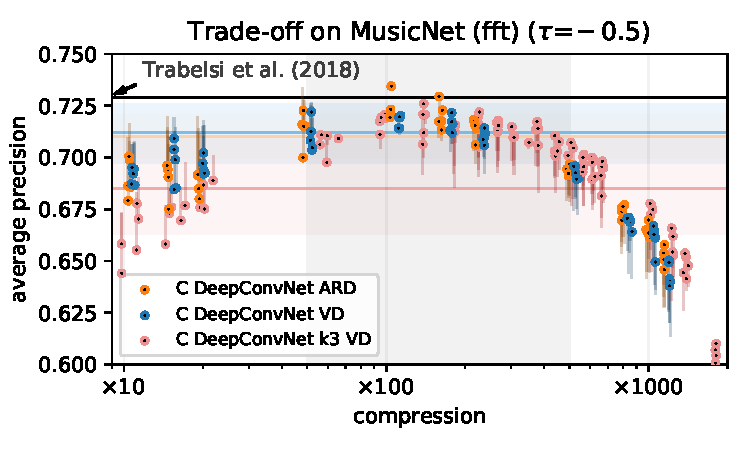
\includegraphics[scale=0.55]{figure__musicnet__trade-off/paper__musicnetram__fft__-0.5.pdf}
  \end{figure}

\end{frame}

% section results_on_musicnet (end)

\section{General Results} % (fold)
\label{sec:general_results}

\begin{frame}[c]{\insertsection}
Experiments on image classification and music transcription
\begin{itemize}
  \item $\cplx$-VD and $\cplx$-ARD equally successfully compress $\cplx$-networks
  \smallskip
  \item Variational Dropout controllably removes redundancy in wide $\cplx$ and $\real$ networks
  \smallskip
  \item $\real$-networks tend to compress better than $\cplx$-nets
\end{itemize}

\bigskip
Compression results are replicable and stable across randomizations
\begin{itemize}
  \item Fine-tuning sparse parameters generally improves performance
\end{itemize}
\end{frame}

% section general_results (end)

\section{Conclusions and Further Developments} % (fold)
\label{sec:conclusions_and_further_developments}

\begin{frame}[c]{\insertsection}
  \begin{columns}[T]
    \begin{column}{0.38\textwidth}
      \begin{itemize}
        \item Extended Bayesian Sparsification method to $\cplx$-valued networks
        \item Empirically explored the compression-performance frontier
      \end{itemize}
    \end{column}
    \begin{column}{0.58\textwidth}
      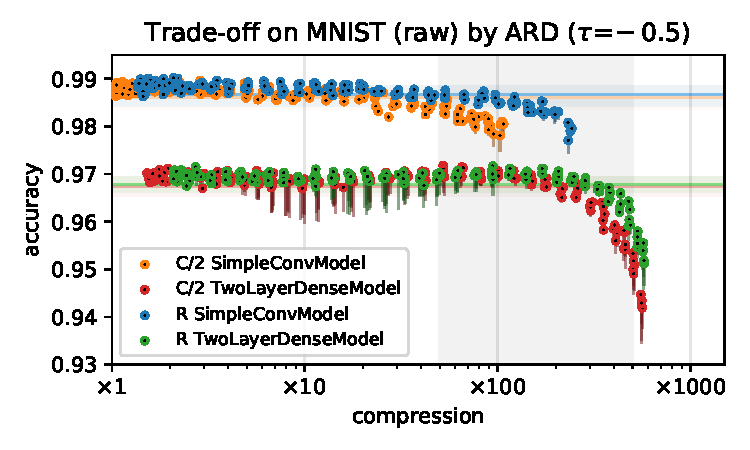
\includegraphics[scale=0.35,clip]{figure__mnist-like__trade-off/appendix__cmp__ARD__mnist__raw__-0.5.pdf}
    \end{column}
  \end{columns}

  \bigskip
  Key limitation: parameter independence % in ${\color{orange} q}$ does not hold in practice
  \begin{itemize}
    \item utilizing parameter coupling may give higher compression
    \item structured sparsity is desirable for SIMD-processing in embedded ML
  \end{itemize}

\end{frame}

% section conclusions_and_further_developments (end)

\section{References} % (fold)
\label{sec:references}

\begin{frame}[c,shrink=35,noframenumbering,plain]{\insertsection}
  \bibliographystyle{abbrvnat}
  \bibliography{presentation}
\end{frame}

% section references (end)

\end{document}
